\documentclass[pdftex,12pt,a4paper]{report}

\usepackage[pdftex]{graphicx}
\usepackage[ansinew]{inputenc}
\usepackage{geometry}
\usepackage{bbold}
\usepackage{program}
\usepackage[toc,page]{appendix}
\usepackage{subcaption}
\geometry{a4paper,left=2.5cm,right=2.5cm, top=2.5cm, bottom=3cm}
\newcommand{\HRule}{\rule{\linewidth}{0.5mm}}

\begin{document}
\begin{titlepage}


%%LR
\sffamily

\begin{center}


% Oberer Teil der Titelseite:

\includegraphics[width=0.3\textwidth]{logo2.jpg}
\hfill

\includegraphics[width=0.4\textwidth]{logo1.jpg}  
\\[5cm]

{\Large Department of Mathematics}\\[0.5cm]
{\Large Chair of Mathematical Modeling of Biological Systems}\\[0.5cm]
{Technische Universit\"at M\"unchen}\\[2cm]
{\Large Master's Thesis in Bioinformatics}\\[1.5cm]

% Title
\HRule \\[0.4cm]
{ \huge \bfseries Single-cell analysis of cancer drug response using computer vision and learning algorithms on time-lapse microtrench data}\\[0.4cm]

\HRule \\[1.5cm]

{\Large Pandu Raharja}\\[2.5cm]

\vfill
\end{center}
\end{titlepage}
\pagestyle{empty}

%%LR comprehensive title
\begin{titlepage}
{\sffamily


\begin{center}

\includegraphics[width=0.3\textwidth]{logo2.jpg}
\hfill

\includegraphics[width=0.4\textwidth]{logo1.jpg}  
\\[1.5cm]  

{\Large Department of Mathematics}\\[0.5cm]
{\Large Chair of Mathematical Modeling of Biological Systems}\\[0.5cm]
{Technische Universit\"at M\"unchen}\\[1cm]

{\Large Master's Thesis in Bioinformatics}\\[2cm]
{\textbf{\Large Single-cell analysis of cancer drug response using computer vision and learning algorithms on time-lapse microtrench data}}\\[2cm]
{\textbf{\Large Wirkungsanalyse von Krebsmedikamenten in Einzeller Aufl\"osung durch die Anwendung von Computer-Vision- und Machine-Learning-Algorithmen auf Microtrench- Videoaufnahme}}\\[4cm]

\end{center}
\begin{center}\Large
  \begin{tabular}{ll}
    Author:& Pandu Raharja\\
    Supervisor: &  Prof. Dr. Fabian Theis, Dr. Carsten Marr\\
    Advisor:        &  Prof. Dr. Fabian Theis\\
    & Prof. Dr. Dmitrij Frishman\\
    Submitted:     &  15.10.2017
  \end{tabular}
\end{center}

}% end title page

\end{titlepage}


%%%%%%%%%%%%%%%%%%%%%%%%%%%%%%%%%
% thesis content starts here
%%%%%%%%%%%%%%%%%%%%%%%%%%%%%%%%%

\newpage


\begin{abstract}
Quantitative measurement of cancer drug response is esential to objectively gauge the efficacy of cancer drugs. So far, there has been no method to track and  quantitatively measure single-cell response of of cancer drug treatment. A novel pipeline is presented in this thesis. First, a quasi-high-throughput method to track cells and quantitatively analyze single-cell response to drugs. We investigate the response of model cancer cell lineagues, MOLM and Jurkat, to known anti-cancer drugs Vincristine and Doxorubicine. While the method enabled relatively easy and quasi-high-throughput analysis of cancer treatment \textit{in vitro}, our pipeline could also be adapted in varios contexts involving single-cell analysis with reasonable amount of modifications necessary.
\end{abstract}

\newpage



\chapter{Introduction}

Lorem ipsum

\chapter{Background}

Lorem ipsum dolor si amet

\chapter{Methods}

\section{Laplacian of Gaussian (LoG) Cell Recognition}

\section{Image Encoding}

Consider whether image encoding shoud contain Lena's picture instead.

\section{Shift Correction}

Consider following picture:

\begin{figure}[h]
\centering
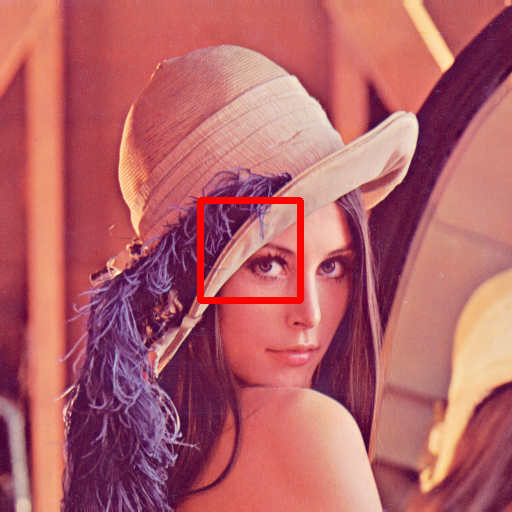
\includegraphics[width=0.5\textwidth]{lenna_marked}
\label{fig:lena}
\caption{Lenna}

\end{figure}

There are many encodings that could be used to internally store this picture. Many such encodings utilized this so-called Red-Green-Blue encodings (RGB). RGB encoding represents the color of a pixel as a combination of red, green and blue color. This encoding is known to various spectra of human visible color and useful enough for most use cases (citation). To give representation on how the encoding works, the RGB encoding of some part of above picture is shown in Figure \ref{fig:lenas}. For an image of size $m \times n$ pixels, the RGB encoding is thus a 4-dimensional matrix of dimension $m \times n \times 3$. For time-lapsed images accordingly, the RGB encoding of the video of length $T$ is a 5-dimensional matrix of shape $t \times m \times n \times 3$.

%An expansion of such encoding, the RGBH encoding, expands the representation by adding the brightness of the pixel -- known as 'hue'.

\begin{figure}[h]
\begin{subfigure}{.5\textwidth}
  \centering
  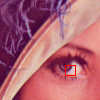
\includegraphics[width=.8\linewidth]{lenna_marked_small}
  \caption{1a}
  \label{fig:lenas1}
\end{subfigure}%
\begin{subfigure}{.5\textwidth}
  \centering
  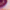
\includegraphics[width=.8\linewidth]{lenna_small}
  \caption{1b}
  \label{fig:lenas2}
\end{subfigure}
\centering
\begin{subfigure}{.5\textwidth}
  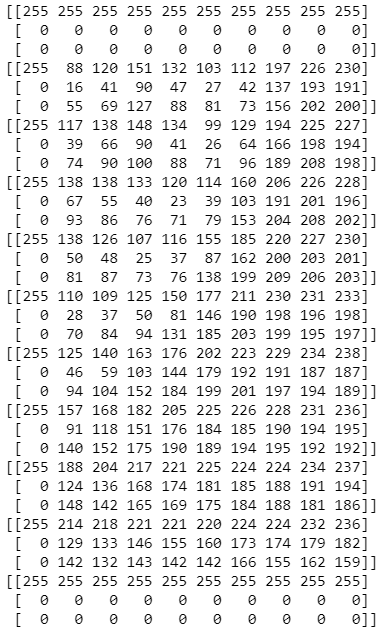
\includegraphics[width=.8\linewidth]{lenna_rbg}
  \caption{1b}
  \label{fig:lenas3}
\end{subfigure}
\caption{Figure \ref{fig:lenas1} shows the content of red marked region in Figure \ref{fig:lena}. Figure\ref{fig:lenas2} shows the zoomed part around Lena's right eye and matrix represented in Figure \ref{fig:lenas3} shows the RGB representation of the eye.}
\label{fig:lenas}
\end{figure}


Now, consider a case in which an image shifts. No rotation of camera is assumed, hence there are only two degree of freedoms (vertical and horizontal). Thus, a shift could be defined as a vector movement $\vec{v}$ of all points $x_{i,j} \in M_{t_i}$ in the time-lapse from time $t_i$ to $t_{i+1}$. Given two degrees of freedom and discreteness of the problem due to pixel representation, the task is reduced to finding difference in x- and y-axis ($\delta_x$ and $\delta_y$), so that the difference of transormed pixels at $t_i$ and the pixels at $t_{i+1}$, i.e.:

$$
argmin_{\delta_x, \delta_y} \{d(M_x, M_y)\}
$$

For distance function $d$, all-channels absolute difference function is used, which is defined as:

$$
d(M, N) = \sum_{c \, \in \, \{R, B, G\}} \sum_{x} \sum_{y} \Vert M_{c, x, y} - N_{c, x, y}\Vert
$$

Since some pixels are lost from the field of view during the view, only a subset of both pictures are used to determine the distance, preferably those around the center point. The search for $(\delta_x, \delta_y)$ pair is then implemented as grid search along x- and y-axis. An example of the search grid is shown in Figure \ref{fig:searchgrid}. In the example, the point that returns the minimum distance was marked with thick black dot and is returned after every grid-search call as inferred shift.\\

\begin{figure}[h]
\centering
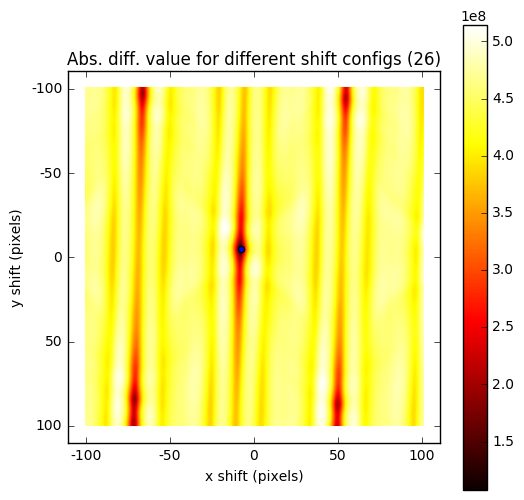
\includegraphics[width=0.5\textwidth]{search_grid}
\caption{Search grid shift for Position 26. The search was conducted for shift between the last time point before and the first time point after the drugs treatment. The minimum is marked with thick black dot. The shift was inferred to be 8 pixels upwards and 5 pixels leftwards. Notice the repeating pattern of relatively favorable configurations after approximately 50 horizontal and 100 vertical pixels caused by lattice nature of the slits.}
\label{fig:searchgrid}
\end{figure}

Since the time-lapsed data consists mainly of grayscale image, the RGB encoding could be the directly transformed to grayscale encoding. Using the transformed method also speeds up the calculation process since the distance function only computes the difference of grayscale channel's values:

$$
d(M, N) =  \sum_{x} \sum_{y} \Vert M_{c, x, y}^{gray} - N_{x, y}^{gray}\Vert
$$

Due to lost pixels around the margin of before and after pictures, only the overlapping part of both slides are included after the correction. Thus, for an inferred shift of $(\delta_x, \delta_y)$, the new dimension of the pictures is then $(m - \delta_x) \times (n - \delta_y)$. This change would then propagation to the other time-lapse images to maintain consistency of the images.

Ideally, the frame correction should be done for each position to reduce the track dropout rate caused by image shifts. This is however computationally very expensive and, as could be seen in Figure \ref{fig:pixdiff}, not really necessary since the biggest shift indeed only happens right before and after the treatment, as it was expected during the experiment setting.

The algorithm for shift inference could be seen in Appendix \ref{appendix:graph}.

\begin{figure}[h]
\centering
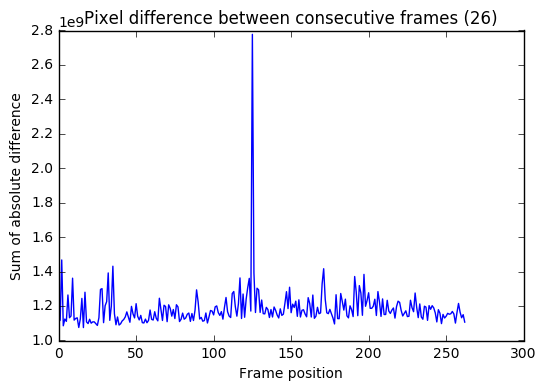
\includegraphics[width=0.8\textwidth]{pixdiff}
\caption{Sum of absolute differences of consecutive stacks for Position 26.}
\label{fig:pixdiff}
\end{figure}

\chapter{Pipeline}
Lorem ipsum

\chapter{Quantitative Analysis}
Lorem ipsum

\chapter{Summary and Outlook}
Lorem ipsum

\begin{appendices}

\chapter{Algorithms}\label{appendix:graph}


\section*{Shift Inference} 

\begin{verbatim}
def infer_shift(last_slide, first_slide, search_space=(200, 200)):
    
  if (search_space[0] % 2 != 0) or (search_space[1] % 2 != 0):
    print("Search spaces have to be even!")
    return None
  else:
    
    ## calculate absolute difference for various shifts
    x1 = search_space[0]
    x2 = search_space[0]
    y1 = search_space[1]
    y2 = search_space[1]
    mid = f1.shape[0] // 2, f1.shape[1] // 2
        
    ## results storage        
    absdiffs = np.zeros((search_space[0] + 1, search_space[1] + 1))

    ## last slide before treatment
    f1sub = f1[(mid[0] - x1):(mid[0] + x2), (mid[1] - y1):(mid[1] + y2)]
    
    ## search space 
    xdiff1 = -int(search_space[0] / 2)
    xdiff2 = int(search_space[0] / 2) + 1
    ydiff1 = -int(search_space[1] / 2)
    ydiff2 = int(search_space[1] / 2) + 1
    
    for xdiff in range(xdiff1, xdiff2):
      for ydiff in range(ydiff1, ydiff2):
      
        ## calculate absolute difference for shift
        f2sub = f2[(mid[0] - x1 + xdiff):(mid[0] + x2 + xdiff), 
                   (mid[1] - y1 + ydiff):(mid[1] + y2 + ydiff)]
        x = xdiff + int(search_space[0] / 2)
        y = ydiff + int(search_space[1] / 2)
        absdiff_xy = np.sum(cv2.absdiff(f1sub, f2sub).ravel())
        absdiffs[x][y] = absdiff_xy
        
        
    ## calculate shift based on calibration data
    x = np.argmin(absdiffs) // absdiffs.shape[0]
    y = np.argmin(absdiffs) % absdiffs.shape[0]
    
    """
    True shift is the opposite of coordinate encoded
    in absdiff
    
    Let X2 the second picture and X1 the first picture.
    If the sub-picture of first slide of X2 centered
    at (c1 + s1, c2 + s2) fits the most with the sub-picture
    of the last slide of X1 centered at (c1, c2)
    then the pictures shift by (-s1, -s2) upon treatment
    """
    diff = -(x - search_space[0] / 2), -(y - search_space[1] / 2)

    return diff
\end{verbatim}

\end{appendices}

\end{document}